\documentclass[11pt,letterpaper]{article}
\usepackage{cogsys}
\usepackage{cogsysapa}
% \usepackage{apacite}
% \usepackage{graphicx}
\usepackage[T1]{fontenc}
\usepackage{times}
\usepackage[pdftex]{graphicx} % use this when importing PDF files
\usepackage{caption}
\usepackage{subcaption}




% Put back in

 % First page headings for accepted submissions.
% \cogsysheading{1}{2012}{1-18}{9/2012}{12/2012}
 % First page headings for poster submissions.
%\cogsysposterheading{First}{2012}{1-18}

% \ShortHeadings{Formatting Instructions}
              % {P.\ Langley, G.\ Hunt, and D.\ G.\ Shapiro}

\begin{document} 

\title{CDSR Human Data/Modelling Paper}
 
% \author{Pat Langley}{langley@asu.edu}
% \author{Glen Hunt}{glen.hunt@asu.edu}
% \address{Computing Science and Engineering, Arizona State University, 
%          Tempe, AZ 85287 USA}
% \author{Daniel G.\ Shapiro}{dgs@isle.org}
% \address{Institute for the Study of Learning and Expertise, 
%          2164 Staunton Court, Palo Alto, CA 94306 USA}
\vskip 0.2in
 
\begin{abstract}
Representing and reasoning about spatial terms is an essential ability for cognitive systems interacting with humans in a shared environment.  Consider an agent asked to remain "in the safe zone" during a military engagement.  The size, shape, and location of this area depend the the capabilities of the agent, other agents in the scene, and the constraints imposed by the environment.  We call these types of regions \textit{context-dependent spatial regions}(CDSRs) due to the context-dependent nature of their extent.  We claim that understanding these regions requires integrating semantic and geometric knowledge about a dynamic environment as well as understanding how task-specific information influences spatial interpretation.  We report the results of a human study conducted to explore how people interpret three types of CDSRs and to support the knowledge integration claim.  We evaluate two representation techniques against the human data and discuss their limitations as a cognitive systems solution to this problem.
\end{abstract}

\section{Introduction - KLENK} 
Natural collaboration between humans and cognitive systems requires both participants to communicate using a shared understanding of spatial language.  Cognitive systems can do quite well with spatial terms defined in terms of coordinates on a map, or that can be specified using known landmarks.  However, many spatial terms are defined not only be their geometry, but also their context and their relevance to current goals.  That is, to understand this language requires considering the other objects and agents in the environment, as well as their configuration and functional roles.  We call such regions \textit{context-dependent spatial regions}(CDSRs).

We begin by discussing the features of CDSRs using illustrative examples.  We claim that (1) people can effectively communicate using these regions, and (2) the size and shape of these regions change with the context.  We argue that to account for this behavior, a cognitive systems solution must respond to changing context, apply learned regions to new situations, and reuse learned knowledge in multiple tasks.  To explore these claims, we present the results of a human study, in which, people marked and rated points and regions for three different environments in 13 different contexts.  In discussing the results, we consider a number of approaches from current cognitive systems and robotics.  Each approach has a number of shortcomings that must be addressed not only to improve our understanding of human spatial reasoning, but also to enable robust intelligent assistants in human environments.

\section{Context-Dependent Spatial Regions}
Consider the following regions (shown in Figure \ref{examples}): the front of a classroom , safety in military engagement, or the geographical feature of a bottleneck.  To identify these regions, one must identify the physical boundaries (e.g., walls), the objects within the room and their functional use (e.g., desks oriented toward a whiteboard), and other agents' intentions and capabilities (e.g., enemy tanks can move and have a range of attack).  Furthermore, these regions exist at different levels of spatial resolution.  Consider a neighborhood in a city, whose boundaries expand and contract overtime with changes to the surrounding residents and businesses.

%Combine these figures into a single figure across
\begin{figure}
\centering
%% Change the classroom to be a picture stimuli
  \begin{subfigure}[b]{0.3\textwidth}
  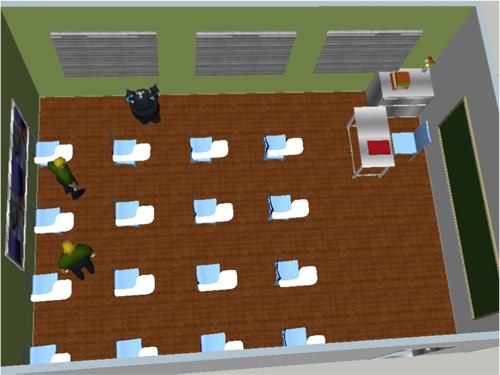
\includegraphics[width=\textwidth]{figures/classroom.png}
  \caption{The front of the classroom is the area between the desks and the whiteboard where people give presentations.}
  \end{subfigure}
\begin{subfigure}[b]{0.3\textwidth}
  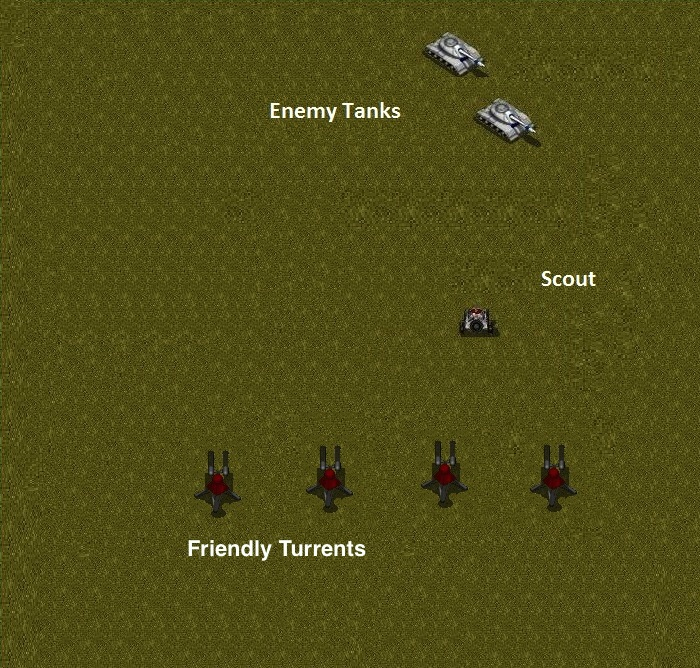
\includegraphics[width=\textwidth]{figures/safety-3.jpg}
  \caption{Safety for the scout is defined by the location of the friendly turrets and the capabilities of the opposing force.}
\end{subfigure}
\begin{subfigure}[b]{0.3\textwidth}
  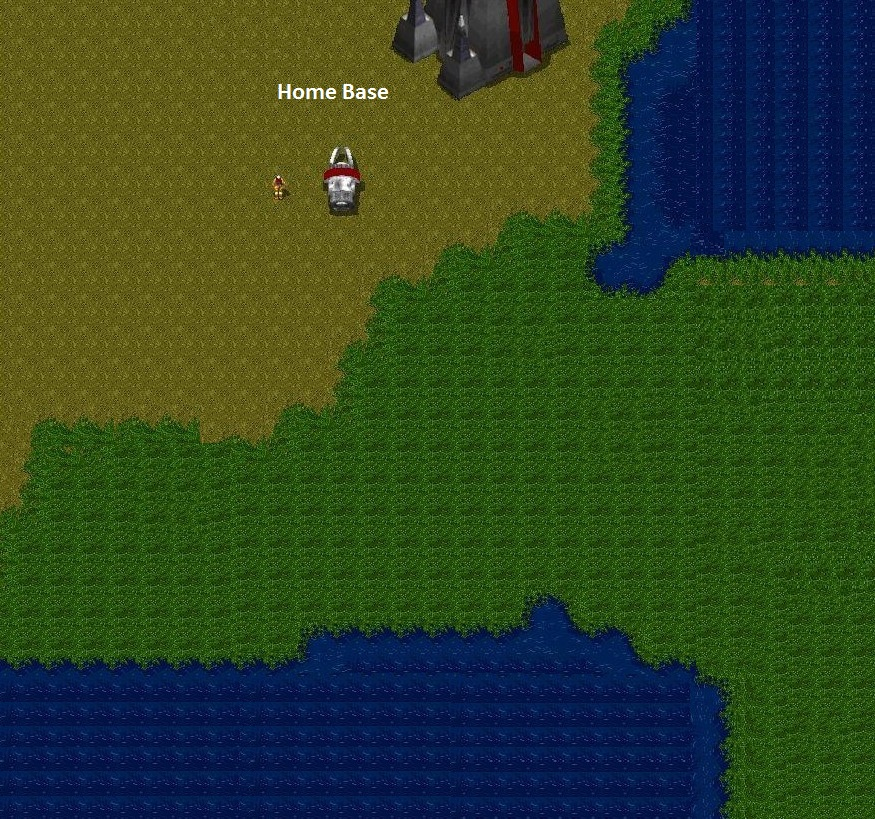
\includegraphics[width=\textwidth]{figures/bottleneck.JPG}
  \caption{A bottleneck occurs when paths are confined to a narrow region by geographic features.  In this case, the water prevents ground movement.}
  \label{fig:safety}
  \end{subfigure}
  
  \caption{Examples of spatial regions used as stimuli in our experiments.}
  \label{fig:examples}
\end{figure}

Understanding these regions is crucial to joint intelligent action with humans.  Not only are these regions frequently tied to goals and commands: "go to the front of the classroom", "defend the bottleneck", and "get to safety", but they are also central to understanding human activities: e.g., "Is there a class in session?".

The long-term goal of this work is to create of agents that can naturally interact with people in human environments.  While the study presented below illustrates the importance of context, object types and configurations, on human spatial judgements, constructing a cognitive systems approach requires more than reproducing these results.  First, the representational approach should be transferable to new situations.  While humans do not demonstrate mastery after a single example of concept, they are able to begin using it immediately refining it over time.  Second, the representation should be applicable in different reasoning tasks.  The functional nature of these regions makes them important for many tasks from action planning to activity recognition.


\section{Human Studies - John}

\subsection{Research Question, Design and Stimuli}

The study was designed to examine the following questions about spatial regions:
\begin{enumerate}
	\item Given a particular situation how well do people agree on the location and extent of a named spatial region?
	\item Does the orientation and location of objects (with relevant functional semantics) in a given situation effect the location and extent of a named spatial region?
\end{enumerate}

To examine these questions we developed three different trials. In all three trial types the subject was presented with a visual stimuli (such as a room floor plan or a map) and an accompanying linguistic description (such as \emph{go to the front of the room}, however the way the task the subject was set varied across the trials:
\begin{enumerate}
	\item Trial type 1: the subject was asked to draw a polygon that defined the extent of the spatial region described in the description or to select a no region option.
	\item Trial type 2: a location was marked on the visual stimuli (using a red x) and the subject was asked to rank on a five point likert scale their judgement of how well the location matched the described spatial region. Three points were pre-selected for each stimuli such that one point was located near the expected prototypical center of the described spatial region and the other two points were at varying distances from this location. The selection of these points was informed by the results of a pilot study. 
	\item Trial type 3: subjects were asked to mark on the visual stimuli, by clicking with the mouse, the location that they felt was most prototypical of the spatial description. 
\end{enumerate}

All three trial types use the same visual stimuli and accompanying spatial descriptions. Figure \ref{fig:exp_stimuli} presents the stimuli used in the experiment. The stimuli can be broken into three groups based on the domain and the spatial region that accompanied them: the classroom domain stimuli were always accompanied by the spatial description \emph{the front of the classroom}; the geographical map stimuli were always accompanied by the description \emph{the bottleneck}; and the military engagement stimuli were always accompanied by the description \emph{safety}. 

The classroom stimuli consisted of pairs of floor plans and photos of classrooms with different chair configurations. For example, Figure \ref{fig:classroom-a} is a floor plan of a classroom where the chairs have been arranged in a circle and Figure \ref{fig:classroom-b} is the accompanying photo of this classroom. We developed four different classroom stimuli each with a different layout of chairs: a circular chair layout, a U shaped layout (Figure \ref{fig:classroom-c} and Figure \ref{fig:classroom-d}), a prototypical layout with the chairs close to the expected front of the room (Figure \ref{fig:classroom-e}), and a prototypical layout with the chairs far away from the expected front of the room (Figure \ref{fig:classroom-f})\footnote{In the interest of saving space we do not show all the classroom photo stimuli}. To control for left-right bias effects two versions of the U shaped layout, close rows layout and far rows layout were created by horizontally flipping the layouts. Conseqeuntly, there were 7 classroom stimuli (circle, U $\times 2$, close $\times 2$, far $\times 2$). In designing these stimuli we deliberately chose some layouts that were very prototypical or close variations on standard layouts - e.g., Figures \ref{fig:classroom-e} and \ref{fig:classroom-f} - and others were more novel - Figure \ref{fig:classroom-a} and \ref{fig:classroom-c}. By varying the prototypicality of the layouts we hoped to get some variation across the between subject agreement on a per stimuli basis, for example we expected to get a higher between subject agreement for the stimuli that were more prototypical. This would provide insight into research question 1, in particular it would point to the effect of prototypicality on the semantics of contextually defined spatial regions. Also, because the prototypicality of the scenes was varied by adjusting the location and orientation of objects in the scenes, a variation in agreement across the stimuli would provide evidence that the orientation and location of objects do effect the location and extent of spatial regions.

The geographical map stimuli, Figures \ref{fig:bottleneck-a} and \ref{fig:bottleneck-b}, differed in the width of the bottleneck region. Finally, the military engagement stimuli, Figures \ref{fig:tanks-a}, \ref{fig:tanks-b}, \ref{fig:turrets-a}, \ref{fig:tanks-b} varied the functionality of the objects in the scene (tanks that could move versus fixed turret emplacements), the location of the objects in the scenes (were the tanks close to the bottom of the image or near the top), and the number and layout of the objects (the number and layout of the turrets were varied). Again, a variation across the between subject agreement on the different stimuli would provide evidence for the impact of object location and orientation on spatial semantics.

\begin{figure}
%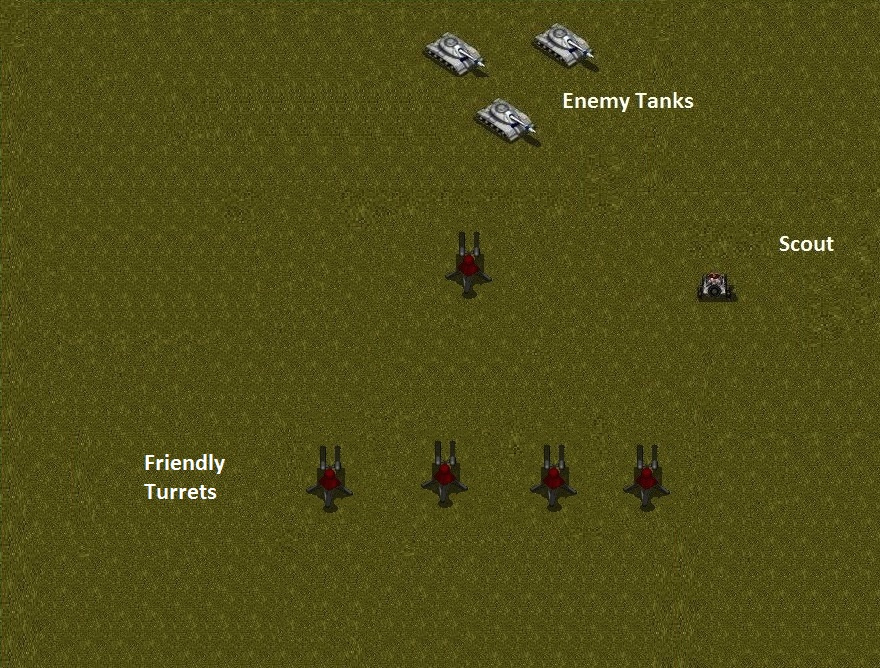
\includegraphics[width=0.4\textwidth]{figures/turrets-plus-one.jpeg}
\centerline{
\begin{tabular}{cccc}
\begin{subfigure}[b]{0.18\textwidth}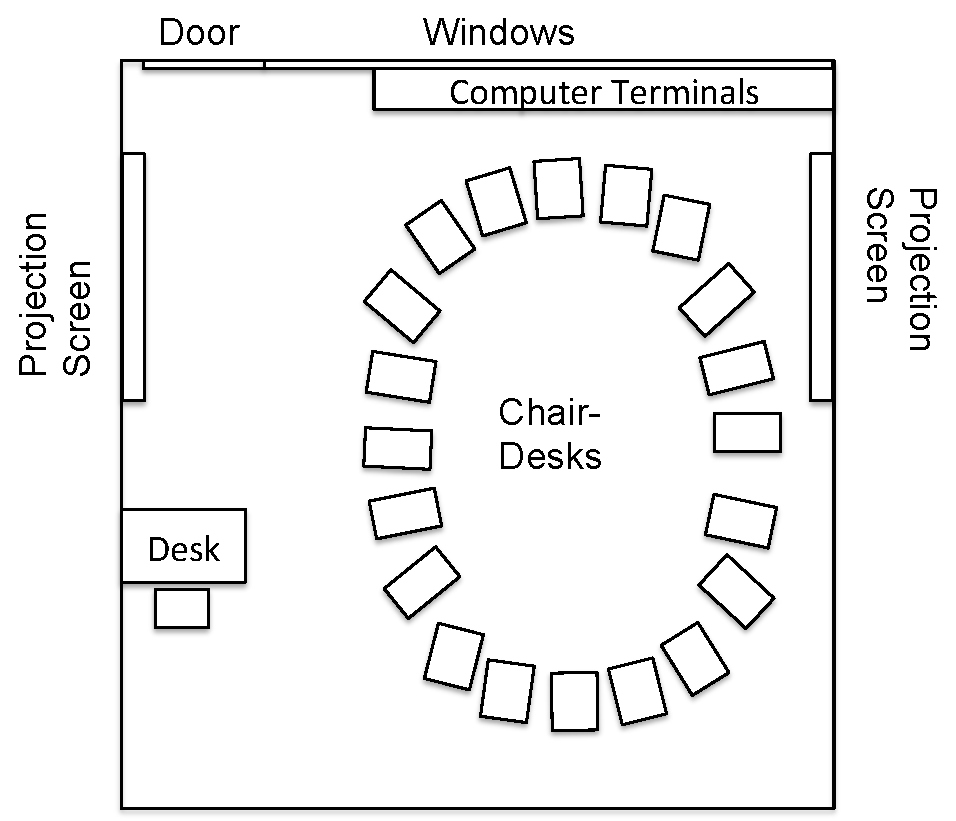
\includegraphics[width=\textwidth]{figures/classroom-circle.pdf}\caption{}\label{fig:classroom-a}\end{subfigure}&
\begin{subfigure}[b]{0.18\textwidth}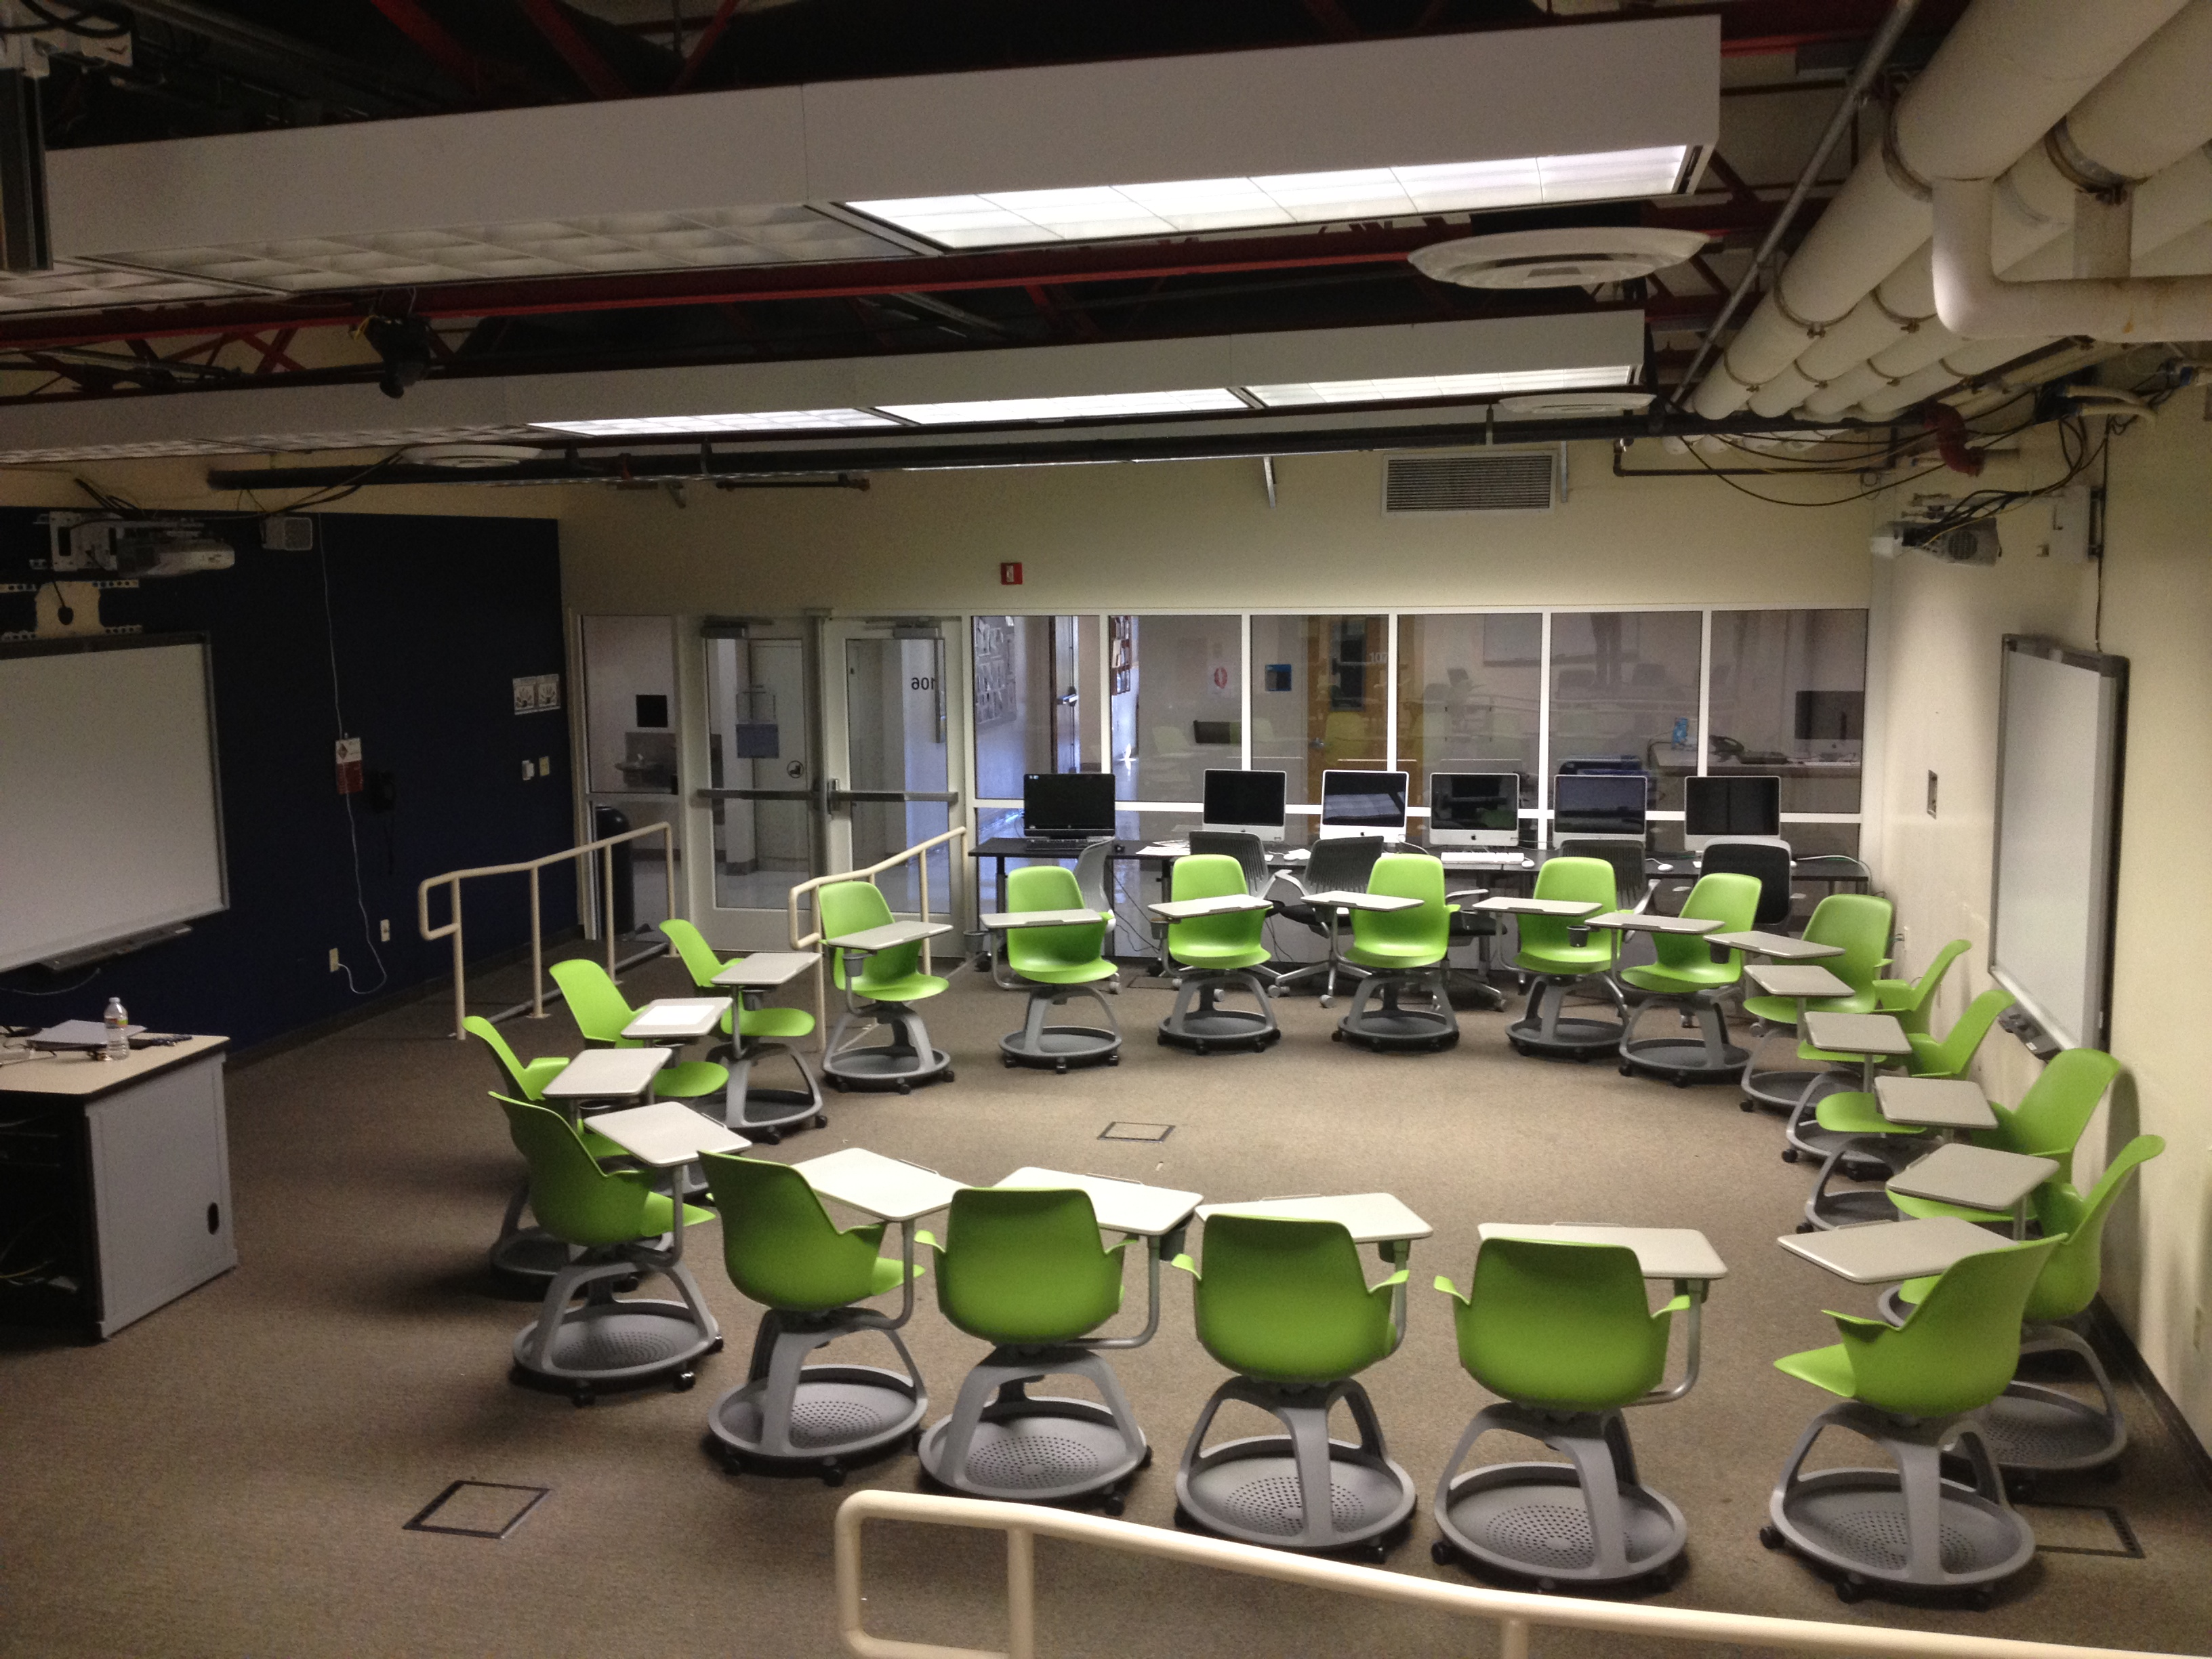
\includegraphics[width=\textwidth]{figures/classroom-circle-photo.jpg}\caption{}\label{fig:classroom-b}\end{subfigure}&
\begin{subfigure}[b]{0.18\textwidth}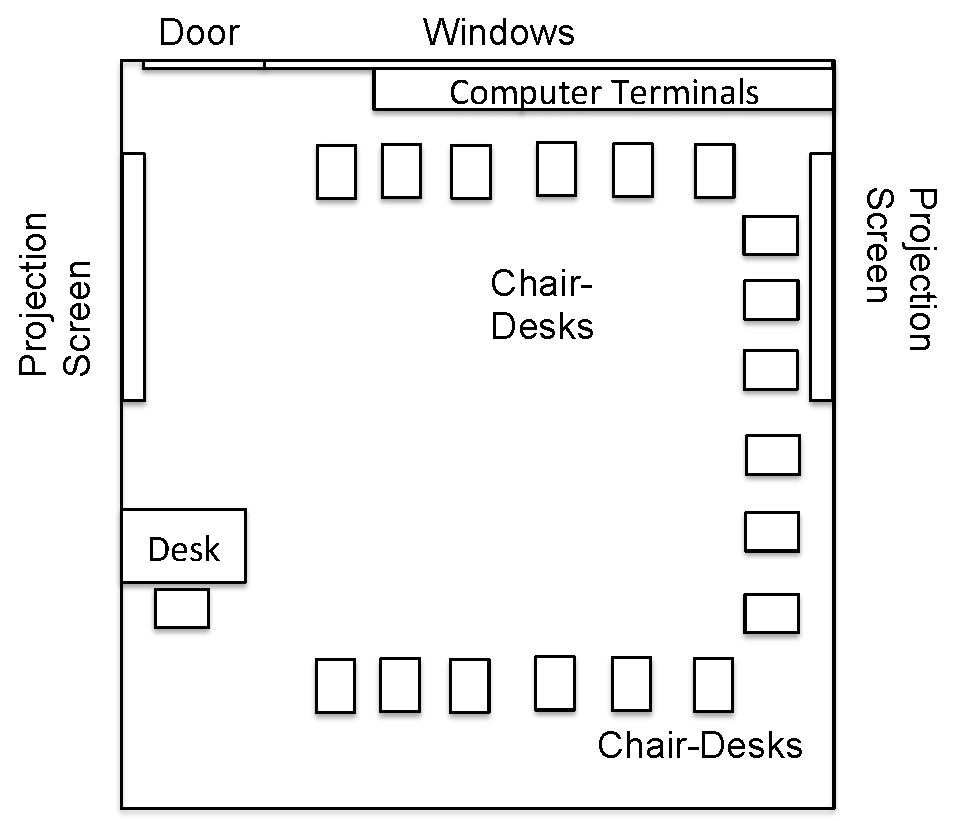
\includegraphics[width=\textwidth]{figures/classroom-u-shaped.pdf}\caption{}\label{fig:classroom-c}\end{subfigure}&
\begin{subfigure}[b]{0.18\textwidth}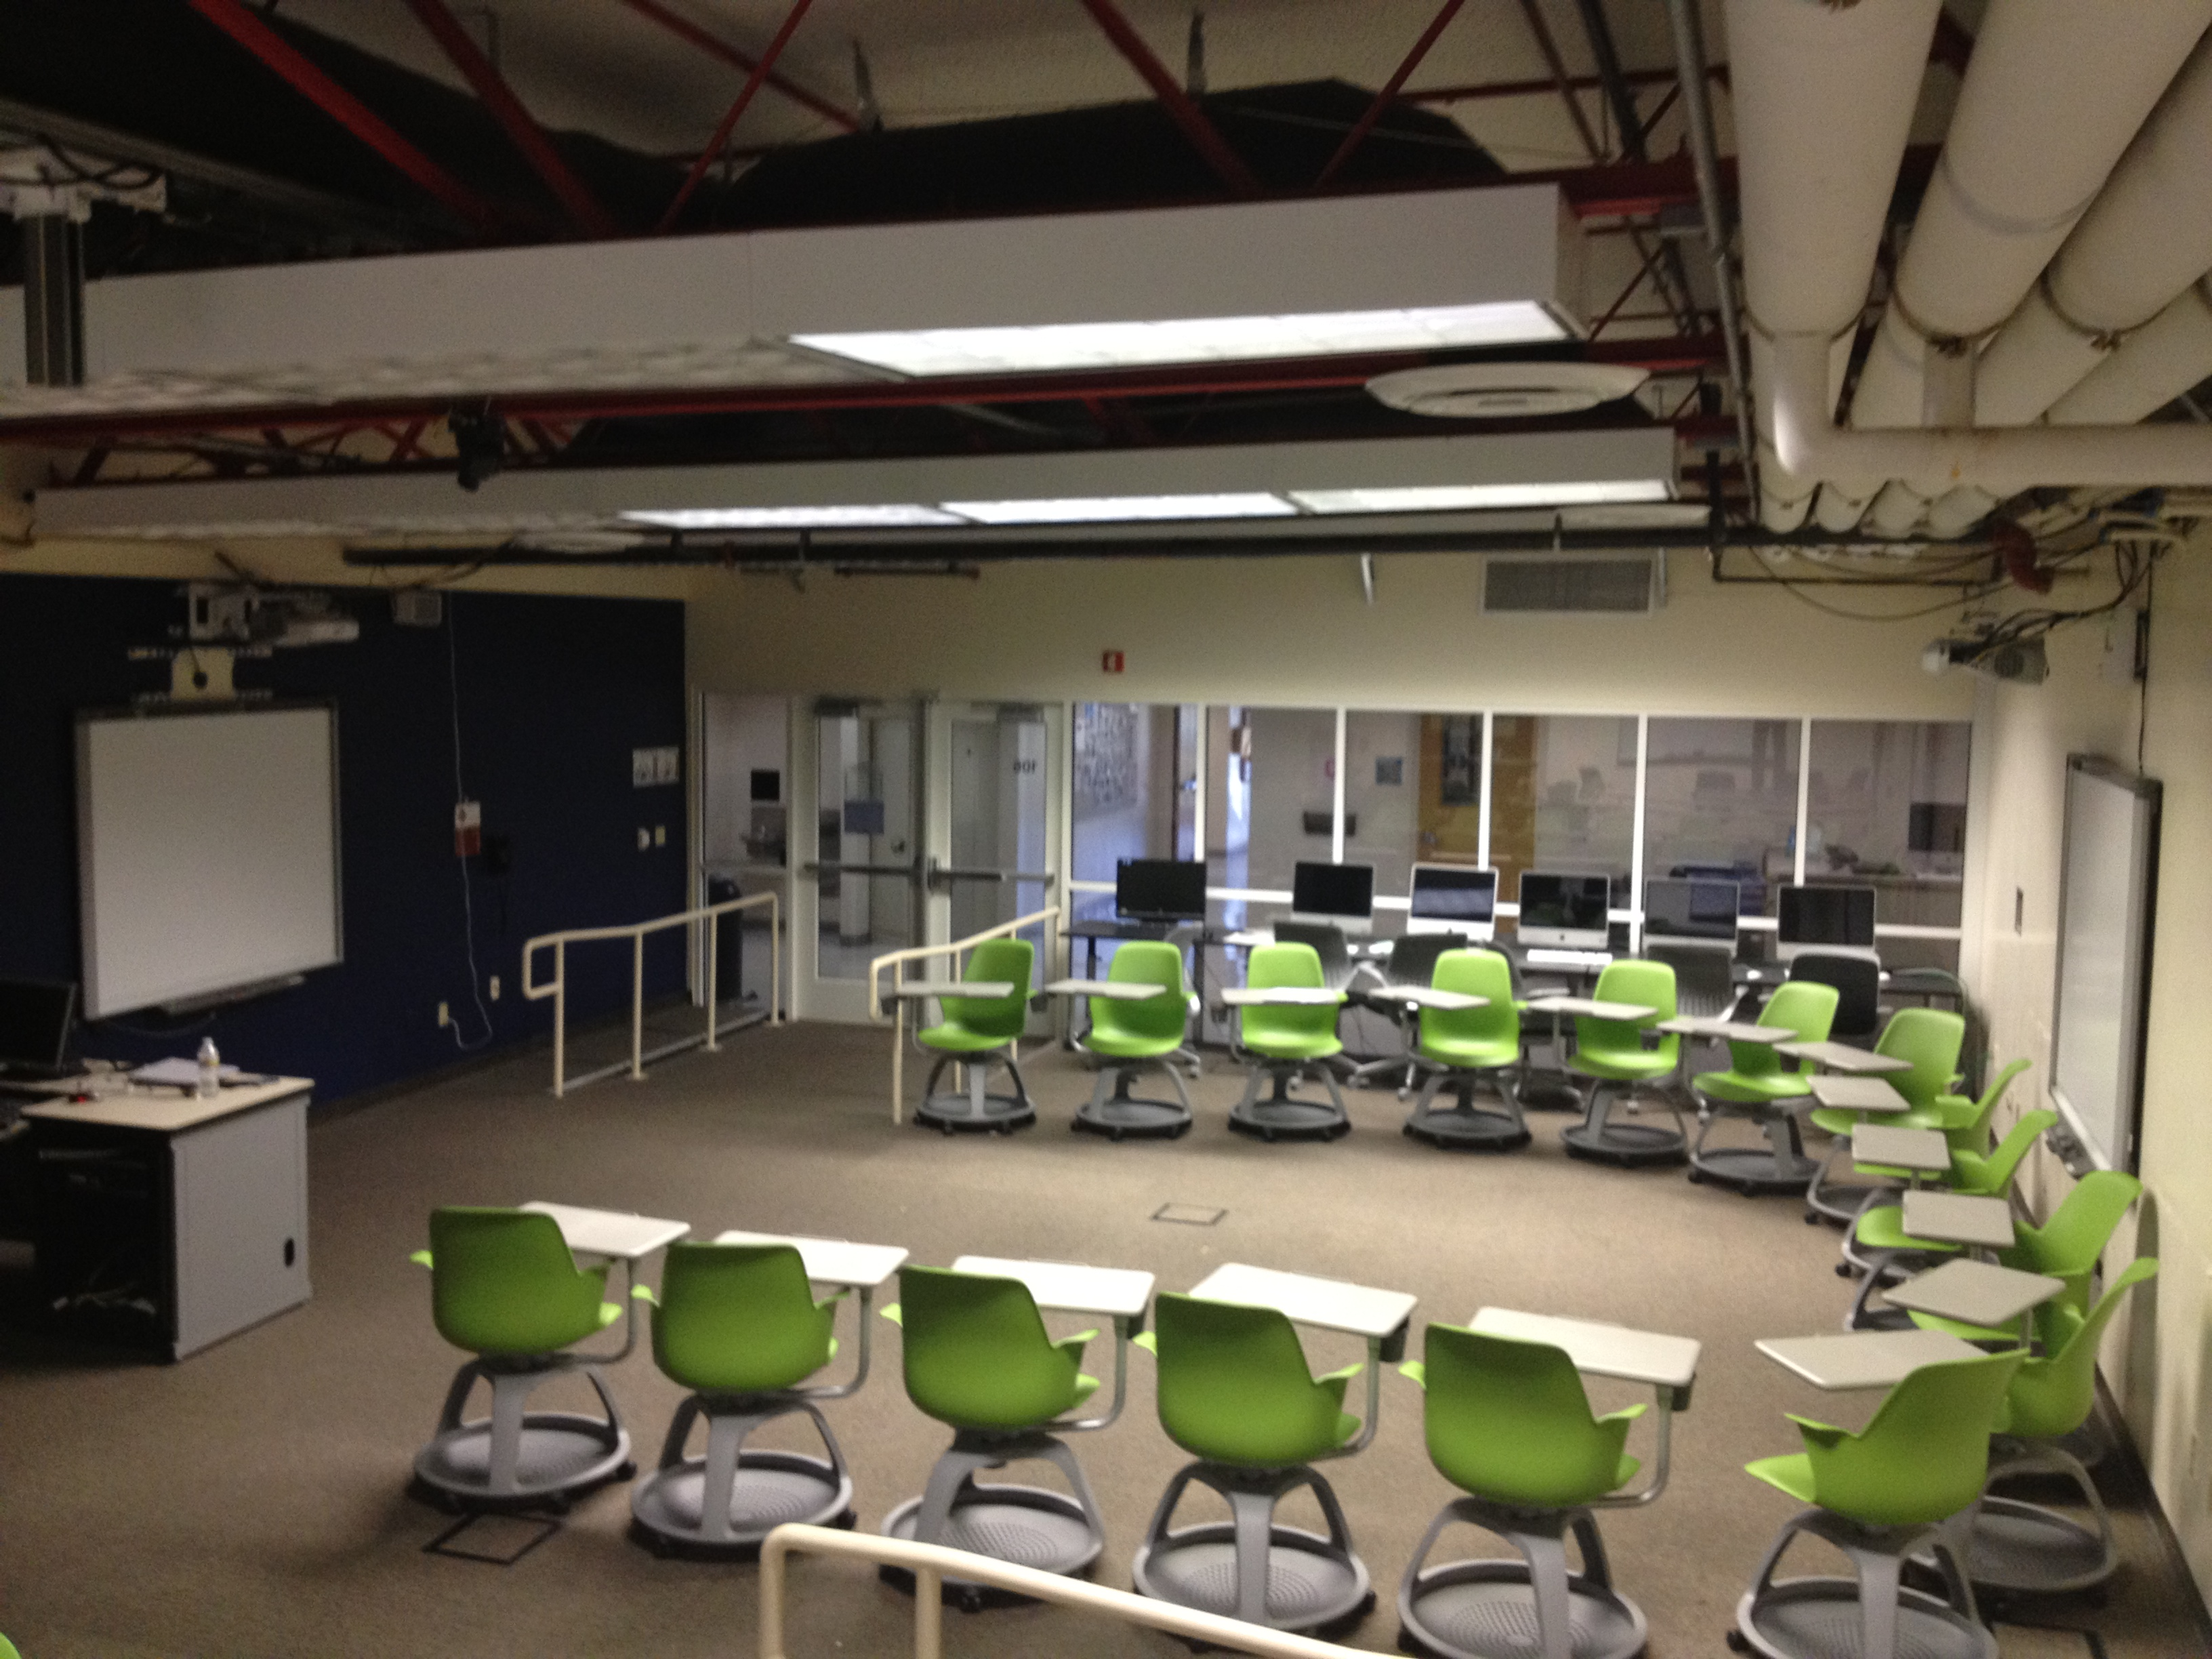
\includegraphics[width=\textwidth]{figures/classroom-u-photo.jpg}\caption{}\label{fig:classroom-d}\end{subfigure}\\
\begin{subfigure}[b]{0.18\textwidth}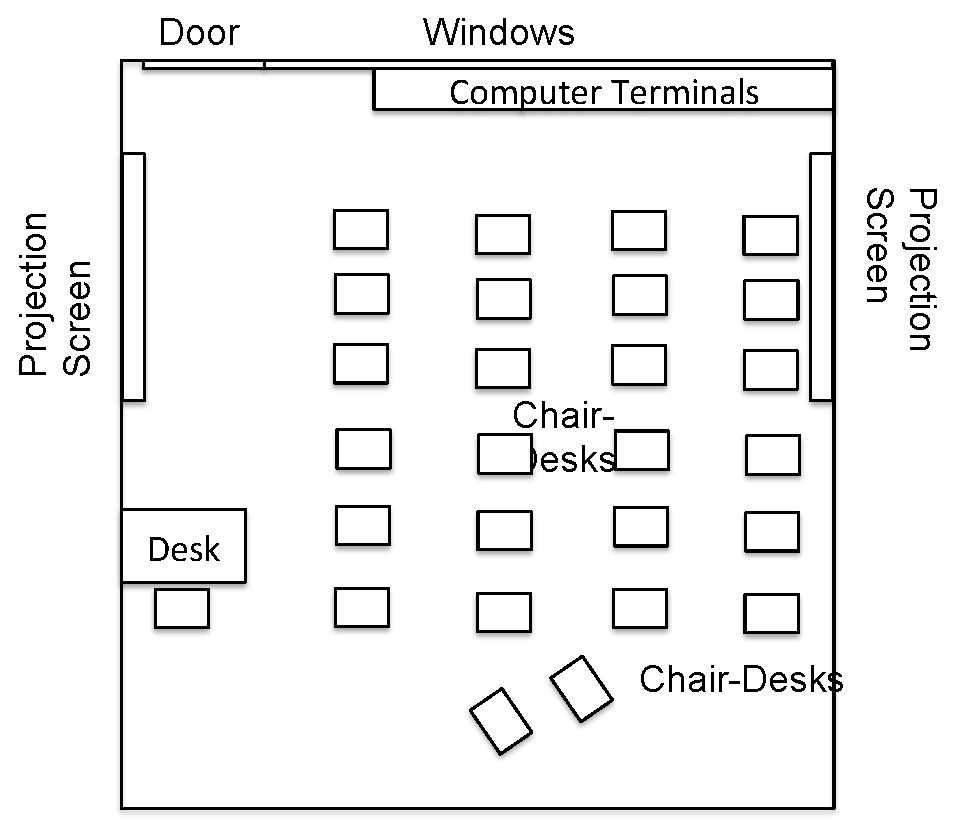
\includegraphics[width=\textwidth]{figures/classroom-close.pdf}\caption{}\label{fig:classroom-f}\end{subfigure}&
\begin{subfigure}[b]{0.18\textwidth}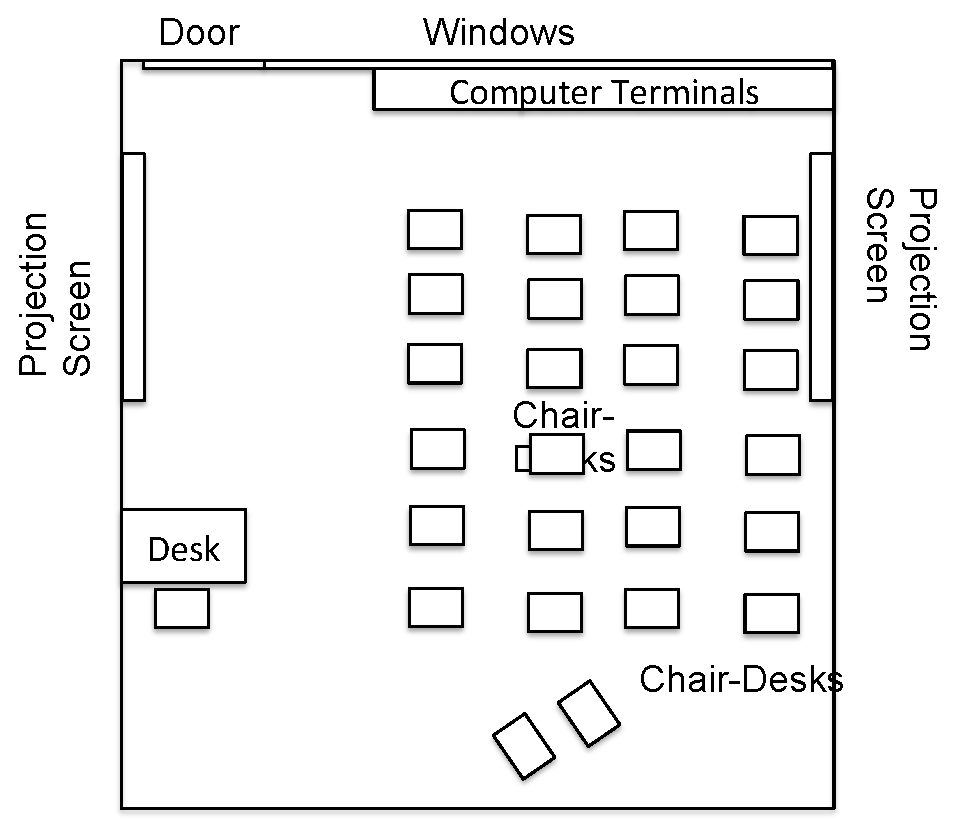
\includegraphics[width=\textwidth]{figures/classroom-far-away.pdf}\caption{}\label{fig:classroom-e}\end{subfigure}&
\begin{subfigure}[b]{0.18\textwidth}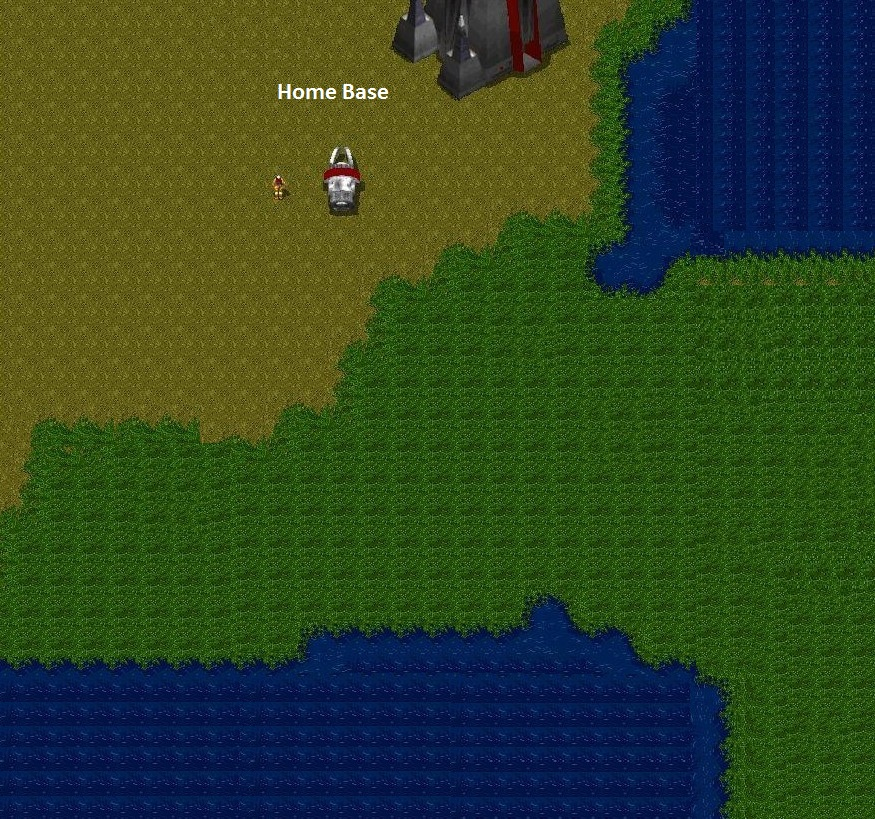
\includegraphics[width=\textwidth]{figures/bottleneck-1.jpg}\caption{}\label{fig:bottleneck-a}\end{subfigure}&
\begin{subfigure}[b]{0.18\textwidth}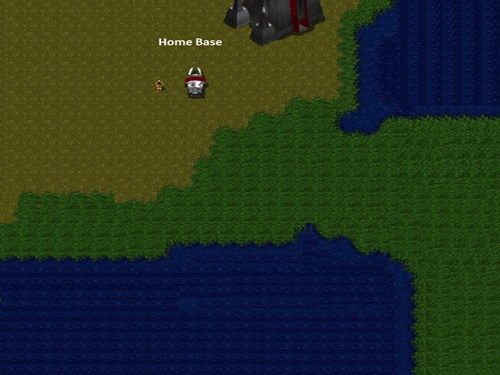
\includegraphics[width=\textwidth]{figures/bottleneck-2.jpg}\caption{}\label{fig:bottleneck-b}\end{subfigure}\\
\begin{subfigure}[b]{0.18\textwidth}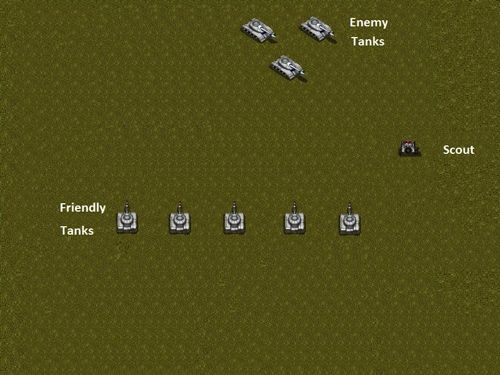
\includegraphics[width=\textwidth]{figures/tanks-close.jpg}\caption{}\label{fig:tanks-a}\end{subfigure}&
\begin{subfigure}[b]{0.18\textwidth}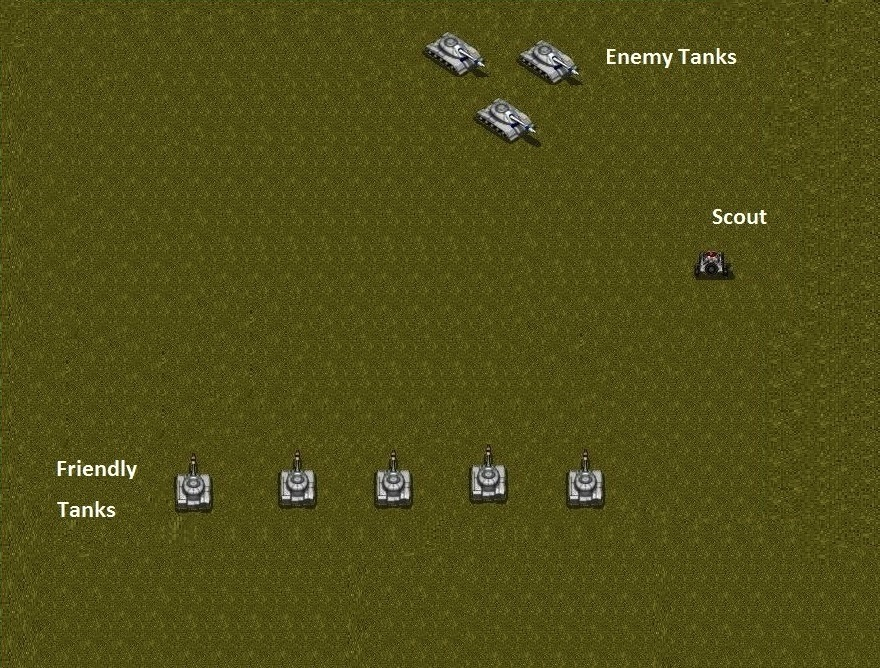
\includegraphics[width=\textwidth]{figures/tanks-far.jpg}\caption{}\label{fig:tanks-b}\end{subfigure}&
\begin{subfigure}[b]{0.18\textwidth}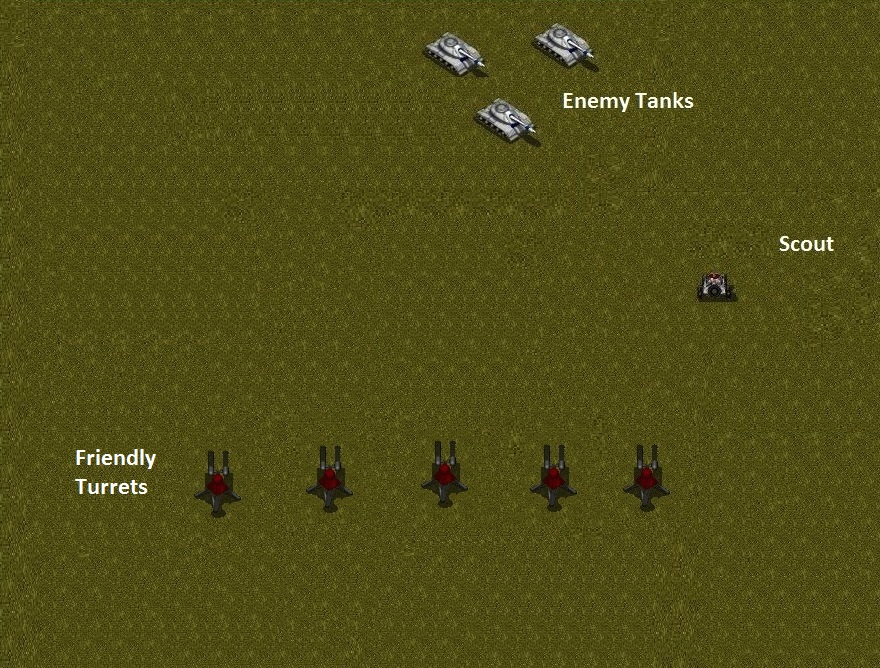
\includegraphics[width=\textwidth]{figures/turrets.jpeg}\caption{}\label{fig:turrets-a}\end{subfigure}&
\begin{subfigure}[b]{0.18\textwidth}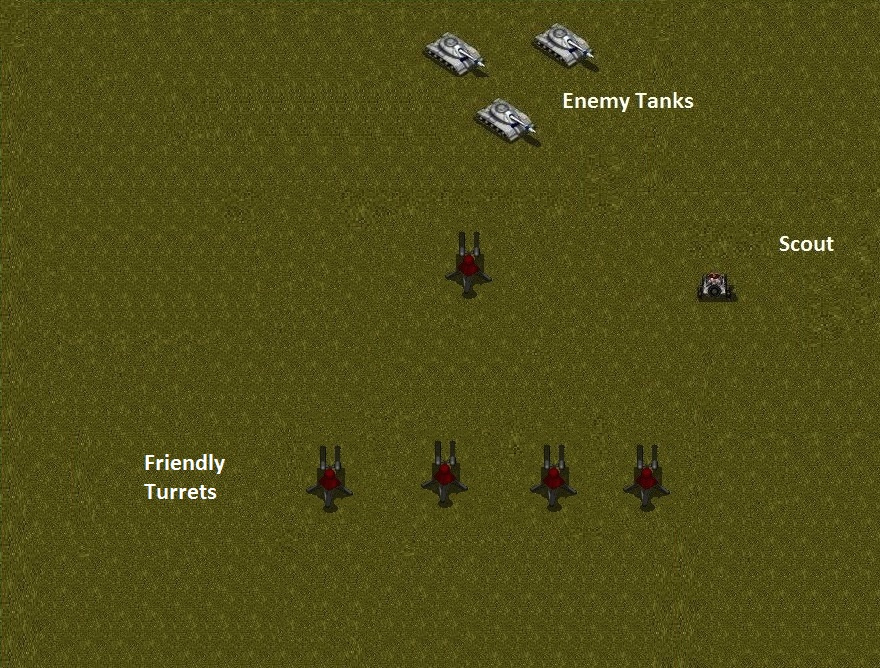
\includegraphics[width=\textwidth]{figures/turrets-plus-one.jpeg}\caption{}\label{fig:turrets-b}\end{subfigure}
\end{tabular}
}
\caption{Experiment Stimuli}
\label{fig:exp_stimuli}
\end{figure}


\subsection{Participants}

43 undergraduate students from two different third level institutes took part in the study. 

\subsection{Analysis}

%Task 1: The participant draws a polygon denoting the region
%Analysis of results:
%(1) Do participants agree/understand-the-task? (validation of approach) + Should anyone be excluded?
%Within the data for each trial,
%-- For each participant, generate the intersection and union polygon of all the other participants
%---- Generate N random points in the area of the full stimulus
%---- For each of these N points check whether the participant's polygon and the [intersection/union] polygon both include it (agree++) or if one includes it and the other doesn't (disagree++)
%---- Then we calculate a Cohen Kappa score as a measure of agreement between the participant and eveyone else. Note we need to calculate the chance of random agreement but we can do this as a function over the relative size of the participant's polygon in the total area of the stimulus and the relative size of the intersection/union polygon
%(see http://en.wikipedia.org/wiki/Cohen%27s_kappa )
%This process will result in for each trial a list of kappa scores for each participant indicating the extent to which they agree with everyone else. We are hoping for a high kappa score
%(2) Does context matter?
%I understand that all the rooms stimuli have the same extent.
%So one way of evaluating whether context matters is to use the kapp score between the intersection/union polygon generated using all the response (less the excluded partitipants) for one trial and the equivalent polygon for another trial.
%We are hoping for a low kappa score

%Cohen's kappa measures the agreement between two annotators who each classify a number of items into two or more mutually exclusive classes as is defined as follows:
%\begin{equation*}
%\kappa = \frac{P(a)-P(ca)}{1-P(ca)}
%\end{equation*}
%where $P(a)$ is the observed relative agreement between the annotators, and $P(ca)$ is the probability of a chance agreement between these to annotators. 
In the type 1 trials subjects drew a polygon on the visual stimuli that defined the location and extent of the relevant spatial region. In analysising the results of these trials we wished to investigate how well the subject's responses agreed with each other and, also, whether the location and orientation of objects in the scene effected the definition of spatial regions in the scene. 

One well known metric for analysising interannotator agreement is the \textbf{Cohen's kappa coefficient}, $\kappa$. Cohen's kappa measures the agreement between two annotators who each classify a number of items into two or more mutually exclusive classes. $\kappa$ ranges from 0 indicating no agreement beyond chance to 1 indicating complete agreement. In order to use Cohen's kappa to measure the agreement between subject responses in our type 1 trials we generated a set of 47,000 test points that were uniformly distribute across each stimuli and used each subject's polygon to classify the test points as being inside or outside the polygon. After classifying the test points for each subject we then computed an average pairwise kappa score for each subject with all the other subjects on a per stimuli basis. In this calculation if either of the subjects in a pair entered a no region response for a particular stimuli a $\kappa$ value of 0 was used. Figure \ref{fig:subj-kappa} shows a histogram of the per subject average kappa scores using ten equal width intervals covering the $\kappa$ range between 0 and 1.  It is evident from this figure that most subjects had a $\kappa$ score between $0.2-0.5$ with a overall majority of subjects having a $\kappa$ score between $0.3-0.4$. A $\kappa$ score between $0.3-0.4$ would be considered as being poor to fair. This would indicate that there was some agreement between subjects but less that would be expected. However, this calculation was done across all the stimuli and as we have already mentioned some of the stimuli were deliberately designed to be non-prototypical, in particular we expected the classroom stimuli where the chairs were arranged in a circle (Figure \ref{fig:classroom-a}) and in a U shaped pattern (Figure \ref{fig:classroom-c} and its horizontally flipped equivalent) to be relatively novel situations for the subjects. Indeed, if we look at the histogram of the average pairwise $\kappa$ scores by stimuli, Figure \ref{fig:stim-kappa}, it is evident that there is a large variation, ranging from $0$ to $0.8$, in $\kappa$ scores for each stimuli. In more detail, Table \ref{tab:stimuli-kappa-scores} lists the average pairwise $\kappa$ score for each of the visual stimuli used in the experiment and the number of no regrion responses for each stimuli. It is clear from this table that the non-prototypical stimuli have the lowest $\kappa$ scores and also that there is relationship between typicality and the number of no region responses. Given this relatively large variation across stimuli, which we attribute to the prototypicality of the depicted situation, we computed the average pairwise $\kappa$ scores for each subject when the non-prototypical stimuli trials were excluded. Figure \ref{fig:subj-kappa-proto} presents the histogram of the resulting average pairwise subject  $\kappa$ scores by subject. Not surpringly, with the exclusion on the non-prototypical stimuli the average pairwise $\kappa$ scores increase, with over half the subjects having an average pairwise $\kappa$ score between $0.4$ and $0.6$. $\kappa$ scores in this range can to interpreted as fair to good.

\begin{figure}
%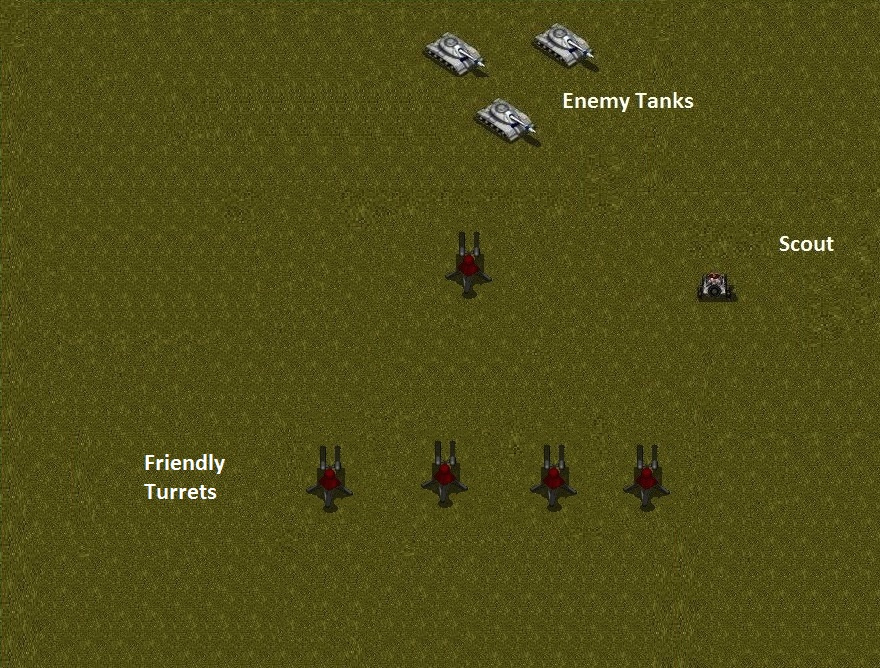
\includegraphics[width=0.4\textwidth]{figures/turrets-plus-one.jpeg}
\centerline{
\begin{tabular}{ccc}
\begin{subfigure}[b]{0.3\textwidth}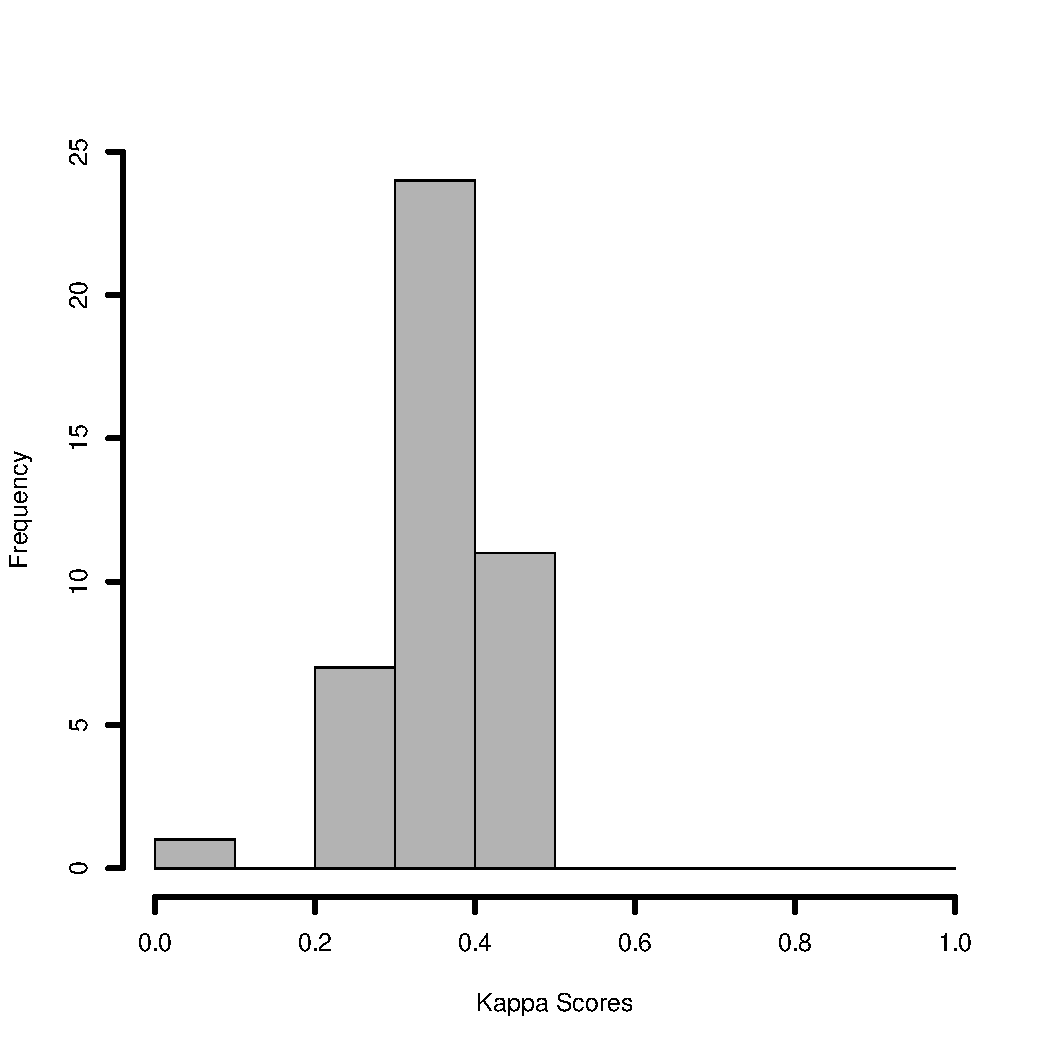
\includegraphics[width=\textwidth]{figures/subj-kappa-hist.pdf}\caption{}\label{fig:subj-kappa}\end{subfigure}&
\begin{subfigure}[b]{0.3\textwidth}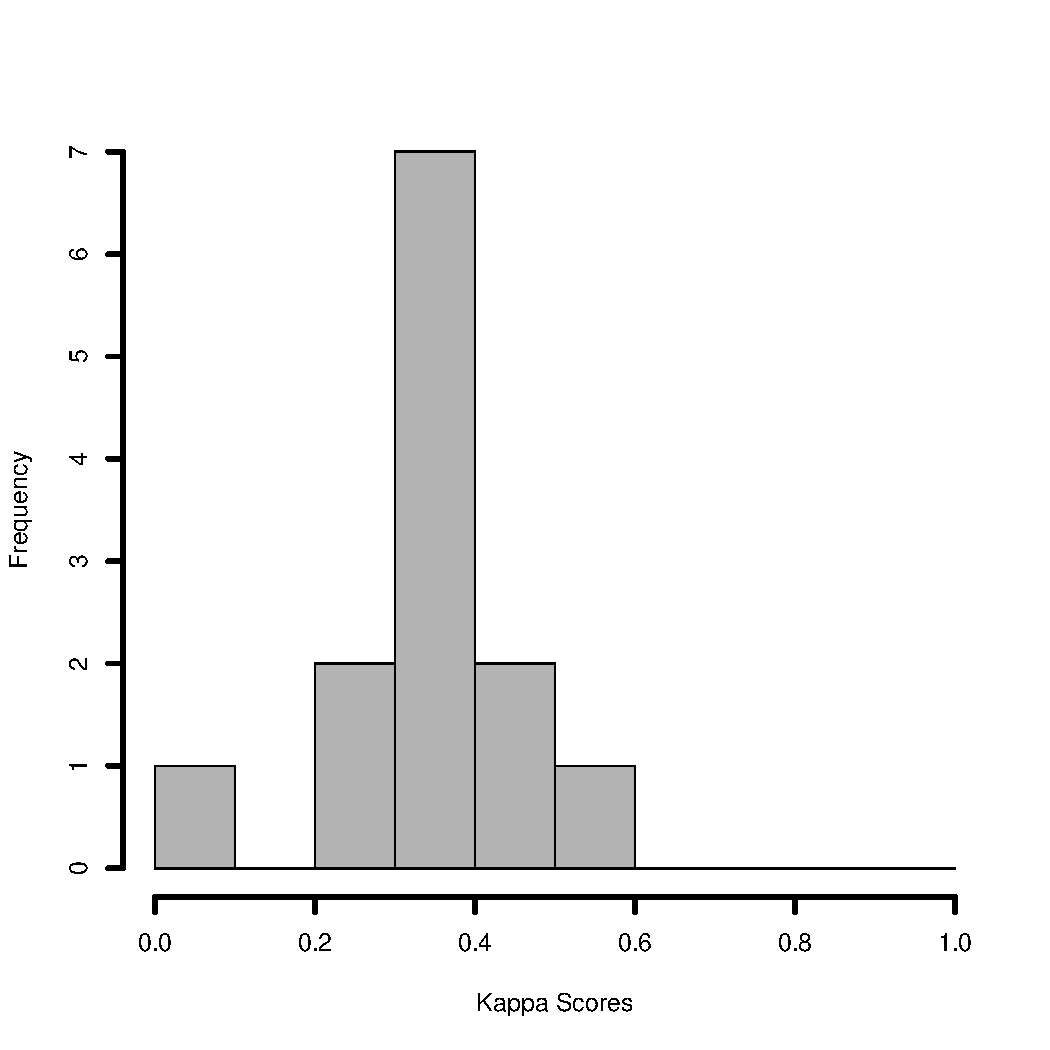
\includegraphics[width=\textwidth]{figures/stimuli-kappa-hist.pdf}\caption{}\label{fig:stim-kappa}\end{subfigure}&
\begin{subfigure}[b]{0.3\textwidth}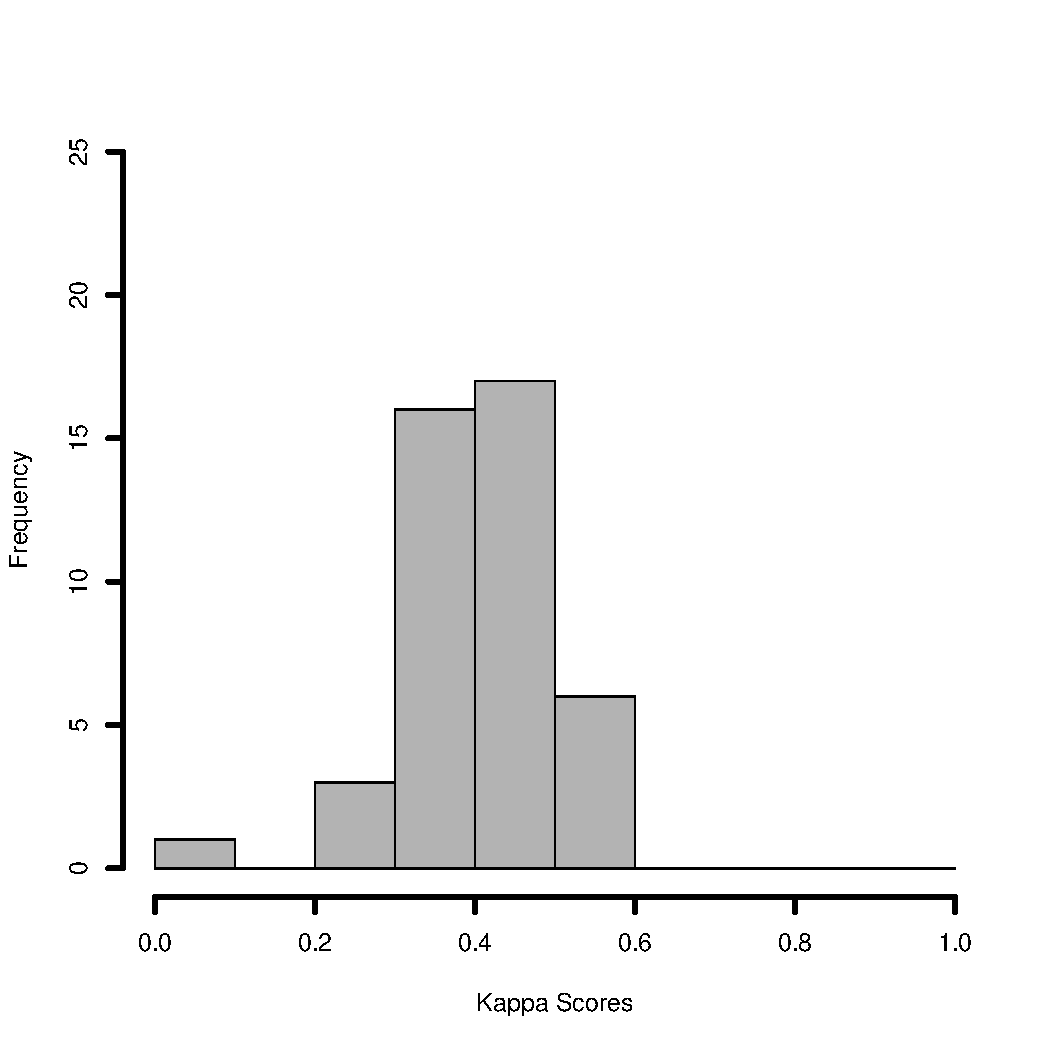
\includegraphics[width=\textwidth]{figures/subj-kappa-hist-protostim.pdf}\caption{}\label{fig:subj-kappa-proto}\end{subfigure}
\end{tabular}
}
\caption{(a) Histogram of average pairwise subject kappa score across all stimuli by subject, (b) histogram of average pairwise subject kappa scores for each stimuli, (c) histogram of average pairwise subject kappa score excluding non-prototypical stimuli by subject.}
\label{fig:type-1-hists}
\end{figure}

\begin{table}
\centerline{
\begin{tabular}{l c c}
Stim ID & Average Pairwise $\kappa$ & No Region Responses\\
\hline
\hline
(h) & 0.5034 & 0\\ % 1_2
(g) & 0.4585 & 1\\ % 1_1
(k) & 0.4548 & 0\\ % 3_3
(f) & 0.3930 & 0\\ % 2_4
(i) & 0.3906 & 0\\ % 3_1
(e-flipped) & 0.3813 & 2\\ % 2_3
(j) & 0.3787 & 1\\ % 3_2
(f-flipped) & 0.3720 & 2\\ % 2_5
(e) & 0.3629 & 1\\ %2_2
(l) & 0.3164& 0\\ % 3_4
(c) & 0.2438 & 2\\ % 2_6
(c-flipped) & 0.2414 & 4\\ %2_7
(a) & 0.0996 & 10 \\ % 2_1
\hline
\end{tabular}
}
\label{tab:stimuli-kappa-scores}
\caption{The average pairwise $\kappa$ scores and the number of no region response by visual stimuli. The stimuli id are based on the labels in Figure \ref{exp-stimuli} with the horizontally flipped versions of stimuli indicated.}
\end{table}


The analysis of the type 1 trials indicates that, over a range of domains and spatial regions, the responses from the subjects did agree, to a good degree. Furthermore, there results support the hypothesis that the defintion of spatial regions in a given context is effected by the location and orientation of objects in the context. For example, focusing on the classroom scenes (stimuli, $a$, $c$, $e$, and $f$) the only difference between these trials was the layout of the chairs in the room and yet there is a substantial variation across these stimuli of the agreement between subjects on the specified spatial region, namely \textit{the front of the room}. Situation $f$ resulted in an average pairwise agreement of $0.393$ and in comparision situation $a$ had an average pairwise agreement of $0.0996$. 


Trial 2
Trial 3

-----------------


-----------------

Task 2: The participant selected a point denoting the sweetspot of the region
Analysis of results:
(1) Do participants agree/understand-the-task? (validation of approach) + Should anyone be excluded?
Compare the variance across the subjects with the variance across a number of set of randomly generate points, where set size equals the number of participants, using the F distribution (http://www.ltcconline.net/greenl/courses/201/regression/comparingVariances.htm) where we are checking if the variance of the random points are greater than that of the participants.
We would hope that the variance of the subjects responses is lower than that of randomly generated points.
After the initial comparison with the random point sets we may exclude participants based on extreme variance.
 
(2) Does context matter?
Do the clusters of participants responses move?
- for each experimental stimulus compute the mean x and y location for the responses for that trial
- check whether the variance between the means of different stimuli responses is greater than the variance within each stimulus responses.

-----------------


Task 3: The participant grades a point with respect to membership of the region on a likert scale
I understand this experiment to be useful because (a) it asks the participants to evaluate (rather than generate cf task 1 and 2) (b) hopefully we can use it to reinforce our findings in task 1 and task 2
I think we need to be careful that the points we present to people for evaluation are reasonably well distributed so that we have a good chance of getting a variation across the responses
Assuming that there is a variation across the likert scores for a particular stimulus then check if their is a correlation between the scores and:
(a) inclusion in the intersection/union polygons from task 1 for the same stimulus
(b) distance from the mean sweet spot for that stimulus from task 2

-----------------
 




\section{Modeling - Nick}


As the results above show, in order for an artificial cognitive system to operate successfully with humans (e.g. understanding spatially-situated task utterances), they must have access to internal models which can represent CDSRs and recognise them in new environments. Whilst spatial reasoning has been an active topic in AI and robotics for decades, CDSRs present a new problem which requires solutions beyond the current state-of-the-art. Regions are central to QSR work~\cite{Cohn:2001}. Regions can either have crisp boundaries, usually defined by geometric shapes (e.g. the bounding boxes of visually tracked objects~\cite{SridharCohn:10}), or vague boundaries created qualitatively by multiple crisp regions (e.g. the `egg-yolk model'~\cite{Cohn96b}), or by thresholding an underlying spatially-mapped function (e.g. those created by potential fields~\cite{brenneretal07ijcai} or by Gaussian kernels~\cite{burbridge-dearden12}). The fundamental decision when creating a computational model of a CDSR is the method used to represent its boundary. Given their context-dependent nature, boundary definitions based purely on single geometric shapes seem unlikely to work. However, arbitrary boundaries can be defined using a sequence of geometric primitives (usually straight lines), as in chain code for image region representations~\cite{Freeman:1961}. This is an approach we followed in previous work, where boundary segments connected vertices defined by contextually-appropriate anchor points~\cite{Hawes:2012}.  Whilst our previous approach provided basic performance, the crisp boundaries it generated caused mismatches with human data over the extent of regions. Methods based on underlying spatial functions may be more flexible in this regard, as they can be selectively thresholded depending on context. 

% Basic approaches

\textbf{TODO:} Perhaps add related work on robot spatial representations, e.g. maps, rooms.  

In the following sections we explore whether two possible CDSR models (one based on boundary segments, one based on a spatial function) are able to satisfy the previously described desiderata for a cognitive systems approach to representing and recognising CDSRs. The surrounding discussion is intended to explore the strengths and weaknesses of these models, providing directions for future research.

\subsection{Symbolic Boundary Method - KLENK}
In our previous work \cite{Hawes:2012}, we presented an approach on a mobile robot that combined qualitative spatial relations, object recognition, and analogy to transfer CDSRs represented as polygons defined by \textit{anchor points} \cite{DBLP:journals/jetai/KlenkFTK11}.  Anchor points are symbolic descriptions that link a conceptual entity (e.g., the front of a classroom) to perceived entities (e.g., the lower left extent of a desk).  An example of the representation and transfer approach is Figure \ref{fig:anchor-point-transfer}.  In the know example, a human defines the front of the classroom as a polygon consisting of four anchor points.  Analogical transfer works by aligning structured representations and transferring partially aligned statements from the known example to the new environment.  In this case, the anchor points are transferred from the group of desks in the known example to the corresponding group of desks in the new environment. 

\begin{figure}
  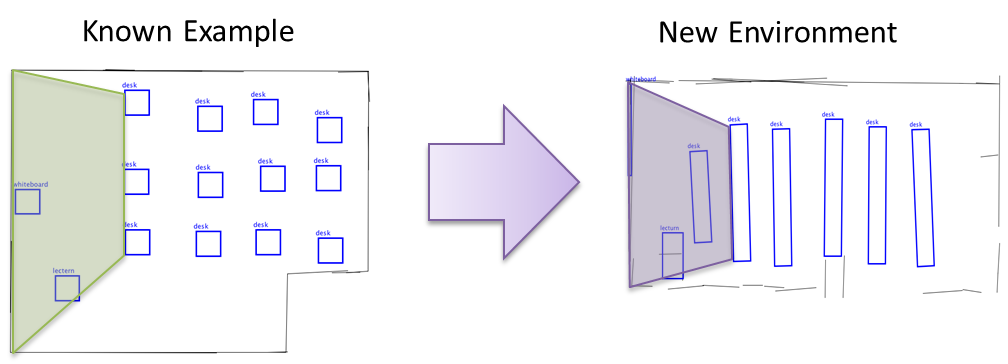
\includegraphics[width=\columnwidth]{figures/classroom-transfer.png}
  \caption{The known example defines the front of the room with four anchor points.  By transferring the anchor points to the new environment, the system is able to ground the room's front in its perception.}
  \label{fig:anchor-point-transfer}
\end{figure}

This method satisfies our criteria for a cognitive systems solution for the following reasons: (1) the alignment process integrates spatial and semantic knowledge about the environment, (2) analogy enables transfer from a single example, (3) while untested, by linking conceptual knowledge to perception, regions defined by anchor points should support any symbolic reasoning task.
 
Applying this model to the points and regions indicated in our experiment illustrates two limitations.  Regions do not always physically bounded by objects.  In the classroom examples, people frequently did not extend the front of the room all way into the corners.  In the safety example, people did not indicate that it was safe behind the lone turret in front of the others.  This indicates that people consider the dynamics of the situation when evaluating these terms, which is not accounted for in this model.

\subsection{Spatial Function Method - NICK}

Overview - either Chris's approach or something similar
Example
Results?
Discussion 
Where do the points come from

\section{Discussion}
 
\begin{acknowledgements} 
\noindent
STRANDS etc.
\end{acknowledgements} 




\vspace{-0.25in}

{\parindent -10pt\leftskip 10pt\noindent
\bibliographystyle{cogsysapa}
\bibliography{cdsr}

}

% Leave a blank line before the closing brace to ensure the final 
% reference has the proper indentation. 

\end{document} 
